\documentclass{article}
\usepackage[utf8]{inputenc}
\usepackage{tikz}
\usepackage{pgfplots}
\pgfplotsset{compat=1.18}
\usetikzlibrary{shapes,arrows,positioning,decorations.pathreplacing}

\title{TikZ Diagrams in LaTeX}
\author{LaTeX Research Toolkit}
\date{\today}

\begin{document}

\maketitle

\section*{Introduction}
This document demonstrates advanced TikZ features for creating complex and visually appealing mathematical graphics and diagrams in \LaTeX. The examples in this document are inspired by Dr. Trefor Bazett's comprehensive TikZ tutorial, which covers everything from basic shapes to advanced node-based diagrams with styled elements and B\'ezier curves.

Key concepts covered include:
\begin{itemize}
    \item Basic shapes and coordinate systems
    \item Styling with colors, fills, and shading
    \item Line styles and arrow variations
    \item Advanced node usage with text and math mode
    \item Relative positioning and anchored nodes
    \item Complex flow diagrams with B\'ezier curves
    \item Reusable custom styles for consistent formatting
\end{itemize}

\subsection*{Setup and Preamble}
To use TikZ in your \LaTeX{} documents, include the following in your preamble:
\begin{verbatim}
\usepackage{tikz}
\usetikzlibrary{positioning}
\end{verbatim}

For advanced features, you may also need additional libraries such as \texttt{shapes}, \texttt{arrows}, and \texttt{decorations.pathreplacing} as shown in this document's preamble. All TikZ commands must be placed inside the \texttt{tikzpicture} environment.

\section{Basic TikZ Examples}
This section covers the fundamental TikZ primitives for drawing shapes using coordinates.

\subsection{Lines and Connections}
Lines are drawn by connecting points using the double dash notation (\texttt{--}):

\begin{center}
\begin{tikzpicture}
% Simple line from point (0,0) to point (4,0)
\draw (0,0) -- (4,0);

% Multi-segment line (polyline)
\draw (5,0) -- (6,1) -- (7,0) -- (8,1);

% Closed shape using cycle
\draw (9,0) -- (10,1) -- (11,0) -- cycle;
\end{tikzpicture}
\end{center}

\subsection{Circles and Ellipses}
Circles are specified by their center point and radius:

\begin{center}
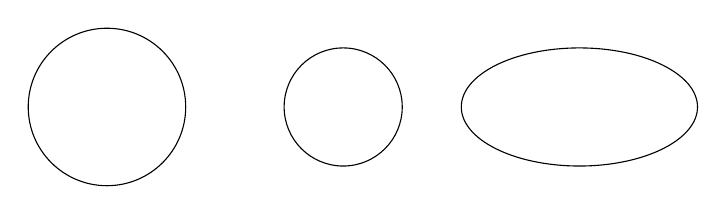
\begin{tikzpicture}
% Circle with center at (0,0) and radius 1cm
\draw (0,0) circle (1cm);

% Circle at different position
\draw (3,0) circle (0.75cm);

% Ellipse with horizontal and vertical radii
\draw (6,0) ellipse (1.5cm and 0.75cm);
\end{tikzpicture}
\end{center}

\subsection{Rectangles and Grids}
Rectangles are drawn by specifying opposite corners:

\begin{center}
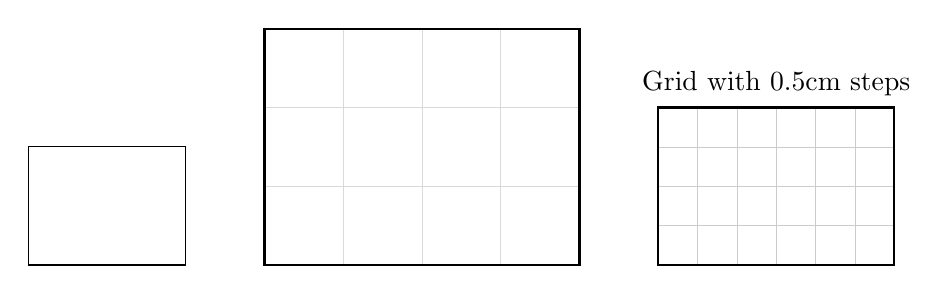
\begin{tikzpicture}
% Rectangle from (0,0) to (2,1.5)
\draw (0,0) rectangle (2,1.5);

% Grid within bounds - useful for coordinate reference
\draw[help lines, gray!30] (3,0) grid (7,3);
\draw[thick] (3,0) rectangle (7,3);

% Labeled grid for reference
\draw[step=0.5cm, gray!40, very thin] (8,0) grid (11,2);
\draw[thick] (8,0) rectangle (11,2);
\node at (9.5, 2.3) {Grid with 0.5cm steps};
\end{tikzpicture}
\end{center}

\subsection{Coordinate System}
\begin{tikzpicture}
% Draw axes
\draw[->] (0,0) -- (4,0) node[right] {$x$};
\draw[->] (0,0) -- (0,4) node[above] {$y$};

% Draw points
\fill (1,1) circle (2pt) node[below right] {$(1,1)$};
\fill (3,2) circle (2pt) node[above left] {$(3,2)$};

% Draw line between points
\draw (1,1) -- (3,2);
\end{tikzpicture}

\section{Styling and Formatting}
This section demonstrates various styling options for TikZ diagrams as shown in Dr. Trefor Bazett's tutorial.

\subsection{Drawing and Styling a Circle}
\begin{center}
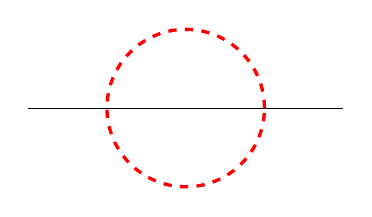
\begin{tikzpicture}
    % Draw a line from (0,0) to (4,0)
    \draw (0,0) -- (4,0);

    % Draw a dashed red circle with a center at (2,0) and a radius of 1cm
    \draw[dashed, red, very thick] (2,0) circle (1cm); 
\end{tikzpicture}
\end{center}

\subsection{Color, Fill, and Shading}
\begin{center}
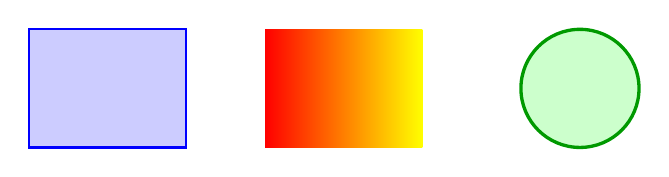
\begin{tikzpicture}
    % Solid fill
    \draw[draw=blue, fill=blue!20, thick] (0,0) rectangle (2,1.5);
    
    % Gradient shading
    \shade[left color=red, right color=yellow] (3,0) rectangle (5,1.5);
    
    % Circle with fill
    \draw[draw=green!60!black, fill=green!20, very thick] (7,0.75) circle (0.75cm);
\end{tikzpicture}
\end{center}

\subsection{Line Styles and Arrows}
TikZ provides extensive options for line styling and arrow configurations:

\begin{center}
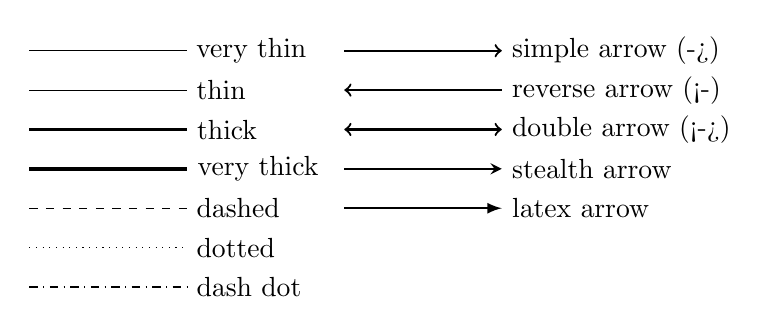
\begin{tikzpicture}
    % Different line thicknesses
    \draw[very thin] (0,3) -- (2,3) node[right] {very thin};
    \draw[thin] (0,2.5) -- (2,2.5) node[right] {thin};
    \draw[thick] (0,2) -- (2,2) node[right] {thick};
    \draw[very thick] (0,1.5) -- (2,1.5) node[right] {very thick};
    
    % Different line patterns
    \draw[dashed] (0,1) -- (2,1) node[right] {dashed};
    \draw[dotted] (0,0.5) -- (2,0.5) node[right] {dotted};
    \draw[dash dot] (0,0) -- (2,0) node[right] {dash dot};
    
    % Arrow variations - add arrows in style brackets
    \draw[->, thick] (4,3) -- (6,3) node[right] {simple arrow (->)};
    \draw[<-, thick] (4,2.5) -- (6,2.5) node[right] {reverse arrow (<-)};
    \draw[<->, thick] (4,2) -- (6,2) node[right] {double arrow (<->)};
    \draw[-stealth, thick] (4,1.5) -- (6,1.5) node[right] {stealth arrow};
    \draw[-latex, thick] (4,1) -- (6,1) node[right] {latex arrow};
\end{tikzpicture}
\end{center}

\subsection{Centering and Scaling}
Graphics can be scaled using the \texttt{scale} parameter or \texttt{transform canvas}:

\begin{center}
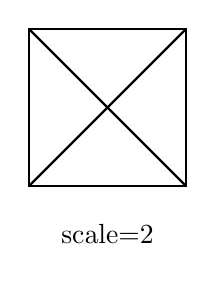
\begin{tikzpicture}[scale=2]
    % Scaled drawing - twice the normal size
    \draw[thick] (0,0) rectangle (1,1);
    \draw[thick] (0,0) -- (1,1);
    \draw[thick] (0,1) -- (1,0);
    \node at (0.5, -0.3) {scale=2};
\end{tikzpicture}
\hspace{1cm}

\begin{tikzpicture}[transform canvas={scale=1.5}]
    % Alternative scaling with transform canvas
    \draw[thick, blue] (0,0) circle (0.5cm);
    \draw[thick, blue] (0,0) -- (0.5,0);
    \node[below] at (0,-0.6) {transform canvas};
\end{tikzpicture}
\end{center}

Both approaches enlarge the graphic, but \texttt{scale} is generally preferred for consistent results. Use the \texttt{center} environment to center graphics in your document.

\section{Advanced Nodes and Positioning}
This section demonstrates advanced node usage. Nodes are highly versatile objects that can contain text and full \LaTeX{} math-mode expressions.

\subsection{Nodes with Text and Math Mode}
Nodes can contain simple text, inline math, and even complex equations using \LaTeX's math capabilities:

\begin{center}
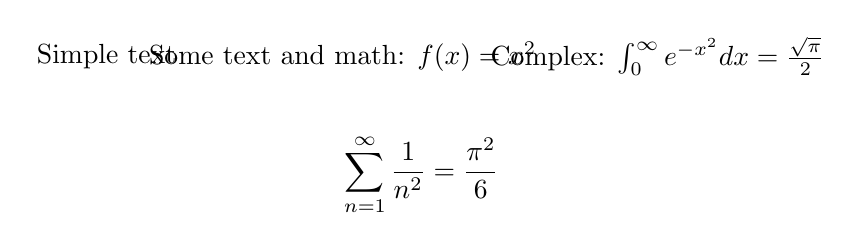
\begin{tikzpicture}
    % Node with simple text
    \node at (0, 0) {Simple text};
    
    % Node with inline math
    \node at (3, 0) {Some text and math: $f(x) = x^2$};
    
    % Node with complex equation
    \node at (7, 0) {Complex: $\int_0^\infty e^{-x^2} dx = \frac{\sqrt{\pi}}{2}$};
    
    % Node with display-style math
    \node at (4, -1.5) {$\displaystyle \sum_{n=1}^{\infty} \frac{1}{n^2} = \frac{\pi^2}{6}$};
\end{tikzpicture}
\end{center}

This powerful feature makes TikZ ideal for creating mathematical diagrams and technical illustrations.

\subsection{Anchored Nodes}
Nodes can be anchored relative to a coordinate or another object using the \texttt{anchor} parameter:

\begin{center}
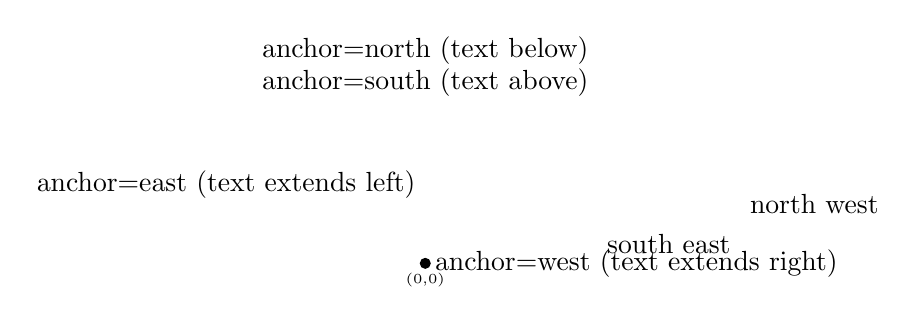
\begin{tikzpicture}
    % Reference point - shown as a dot
    \fill (0,0) circle (2pt) node[below, font=\tiny] {(0,0)};
    
    % Nodes anchored at different positions relative to the point
    \node[anchor=west] at (0,0) {anchor=west (text extends right)};
    \node[anchor=east] at (0,1) {anchor=east (text extends left)};
    \node[anchor=south] at (0,2) {anchor=south (text above)};
    \node[anchor=north] at (0,3) {anchor=north (text below)};
    
    % Diagonal anchors
    \node[anchor=south east] at (4,0) {south east};
    \node[anchor=north west] at (4,1) {north west};
\end{tikzpicture}
\end{center}

Understanding anchors is crucial for precise node placement and alignment in complex diagrams.

\subsection{SIR Model Diagram with Styled Nodes}
This example demonstrates the SIR (Susceptible-Infected-Recovered) epidemiological model using styled nodes and relative positioning. This showcases how to:
\begin{itemize}
    \item Define custom reusable styles
    \item Position nodes relatively using \texttt{below of}
    \item Connect nodes using their anchors (e.g., \texttt{.south}, \texttt{.north})
    \item Add labels to arrows using \texttt{node[midway]}
\end{itemize}

\begin{center}
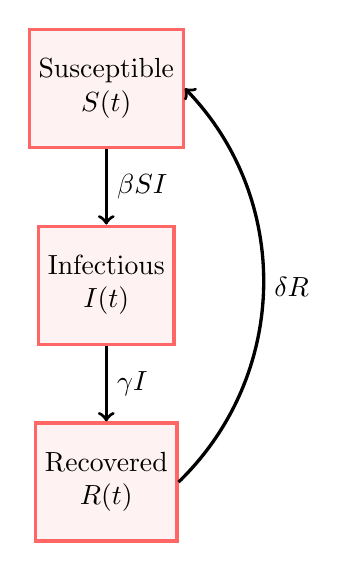
\begin{tikzpicture}[
    sir/.style={
        rectangle, 
        draw=red!60!white, 
        fill=red!5!white, 
        very thick, 
        minimum size=1.5cm,
        align=center
    },
    node distance=2.5cm 
]

    % Create nodes with relative positioning
    % First node (Susceptible) - reference position
    \node[sir] (susceptible) {Susceptible \\ $S(t)$}; 

    % Second node (Infectious) positioned below the first
    \node[sir, below of=susceptible] (infectious) {Infectious \\ $I(t)$};
    
    % Third node (Recovered) positioned below the second
    \node[sir, below of=infectious] (recovered) {Recovered \\ $R(t)$};

    % Connect nodes using their anchors with labeled arrows
    \draw[->, very thick] (susceptible.south) -- (infectious.north) 
        node[midway, right] {$\beta SI$};
    \draw[->, very thick] (infectious.south) -- (recovered.north) 
        node[midway, right] {$\gamma I$};
    
    % Add a curved arrow using Bézier curve (loss of immunity)
    \draw[->, very thick] (recovered.east) to[bend right=45] 
        node[right] {$\delta R$} (susceptible.east);

\end{tikzpicture}
\end{center}

The positioning library is required for \texttt{below of} and similar commands.

\subsection{Curved Arrows with B\'ezier Curves}
B\'ezier curves allow you to create smooth curves by specifying control points. The syntax is: \texttt{.. controls (x1,y1) and (x2,y2) ..}

\begin{center}
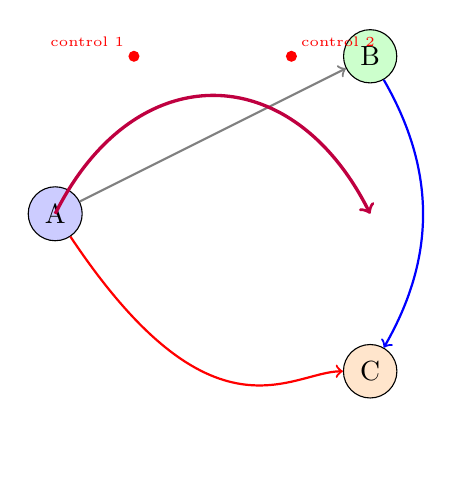
\begin{tikzpicture}
    % Define nodes
    \node[circle, draw, fill=blue!20] (A) at (0,0) {A};
    \node[circle, draw, fill=green!20] (B) at (4,2) {B};
    \node[circle, draw, fill=orange!20] (C) at (4,-2) {C};
    
    % Straight arrow for reference
    \draw[->, thick, gray] (A) -- (B);
    
    % Curved arrow using Bézier curve with explicit control points
    % The curve passes through (A) and (C), shaped by controls at (2,-3) and (3,-2)
    \draw[->, thick, red] (A) .. controls (2,-3) and (3,-2) .. (C);
    
    % Smooth curve using 'to' notation with bend
    \draw[->, thick, blue] (B) to[bend left=30] (C);
    
    % More complex Bézier curve showing control points
    \draw[->, very thick, purple] (0,0) .. controls (1,2) and (3,2) .. (4,0);
    
    % Show control points for illustration
    \fill[red] (1,2) circle (2pt) node[above left, font=\tiny] {control 1};
    \fill[red] (3,2) circle (2pt) node[above right, font=\tiny] {control 2};
\end{tikzpicture}
\end{center}

The control points determine the shape and direction of the curve. Experiment with different positions to achieve the desired curve.

\subsection{Complex Flow Diagram with Relative Positioning}
\begin{center}
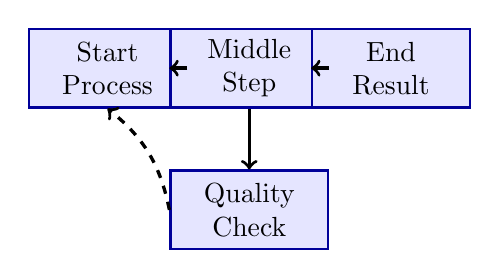
\begin{tikzpicture}[
    box/.style={rectangle, draw=blue!60!black, fill=blue!10, thick, minimum width=2cm, minimum height=1cm, align=center},
    node distance=1.8cm
]
    % Create nodes with relative positioning
    \node[box] (start) {Start \\ Process};
    \node[box, right of=start] (middle) {Middle \\ Step};
    \node[box, right of=middle] (end) {End \\ Result};
    \node[box, below of=middle] (check) {Quality \\ Check};
    
    % Connect nodes with arrows
    \draw[->, very thick] (start) -- (middle);
    \draw[->, very thick] (middle) -- (end);
    \draw[->, very thick] (middle) -- (check);
    \draw[->, very thick, dashed] (check.west) to[bend right=20] (start.south);
\end{tikzpicture}
\end{center}

\section{Flowcharts}
Here's a simple flowchart:

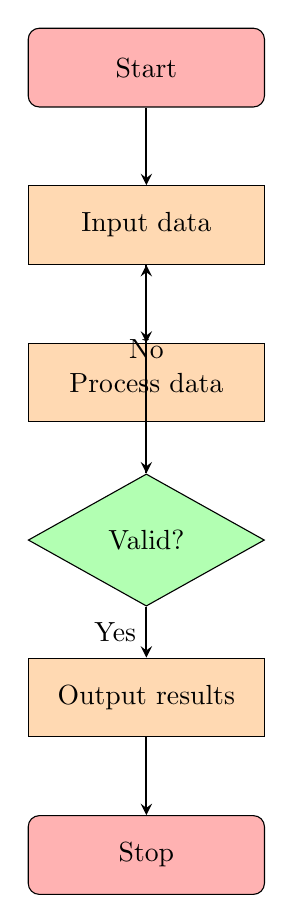
\begin{tikzpicture}[node distance=2cm]
% Define styles
\tikzstyle{startstop} = [rectangle, rounded corners, minimum width=3cm, minimum height=1cm, text centered, draw=black, fill=red!30]
\tikzstyle{process} = [rectangle, minimum width=3cm, minimum height=1cm, text centered, draw=black, fill=orange!30]
\tikzstyle{decision} = [diamond, minimum width=3cm, minimum height=1cm, text centered, draw=black, fill=green!30]
\tikzstyle{arrow} = [thick,->,>=stealth]

% Draw nodes
\node (start) [startstop] {Start};
\node (input) [process, below of=start] {Input data};
\node (process) [process, below of=input] {Process data};
\node (decision) [decision, below of=process] {Valid?};
\node (output) [process, below of=decision] {Output results};
\node (stop) [startstop, below of=output] {Stop};

% Draw arrows
\draw [arrow] (start) -- (input);
\draw [arrow] (input) -- (process);
\draw [arrow] (process) -- (decision);
\draw [arrow] (decision) -- node[anchor=east] {Yes} (output);
\draw [arrow] (decision) -- node[anchor=south] {No} (input);
\draw [arrow] (output) -- (stop);
\end{tikzpicture}

\section{Mathematical Plots}
Here's a mathematical plot:

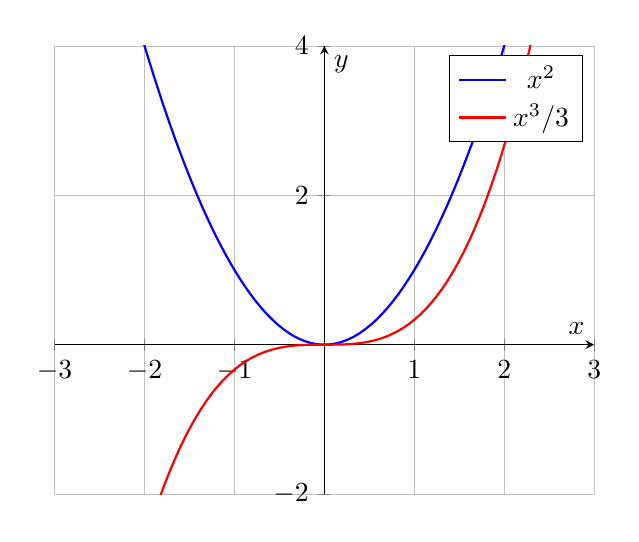
\begin{tikzpicture}
\begin{axis}[
    axis lines = center,
    xlabel = $x$,
    ylabel = $y$,
    xmin = -3, xmax = 3,
    ymin = -2, ymax = 4,
    grid = both,
    grid style = {line width=.1pt, draw=gray!10},
    major grid style = {line width=.2pt, draw=gray!50},
]
\addplot[domain=-3:3, samples=100, color=blue, thick] {x^2};
\addplot[domain=-3:3, samples=100, color=red, thick] {x^3/3};
\legend{$x^2$, $x^3/3$}
\end{axis}
\end{tikzpicture}

\section{Network Diagrams}
Here's a simple network diagram:

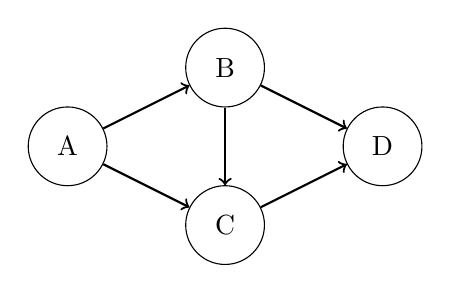
\begin{tikzpicture}[node distance=2cm]
% Define node styles
\tikzstyle{node} = [circle, draw, minimum size=1cm]
\tikzstyle{edge} = [thick, ->]

% Draw nodes
\node[node] (A) at (0,0) {A};
\node[node] (B) at (2,1) {B};
\node[node] (C) at (2,-1) {C};
\node[node] (D) at (4,0) {D};

% Draw edges
\draw[edge] (A) -- (B);
\draw[edge] (A) -- (C);
\draw[edge] (B) -- (D);
\draw[edge] (C) -- (D);
\draw[edge] (B) -- (C);
\end{tikzpicture}

\section{Advanced TikZ Features}
Here are some advanced TikZ features:

\subsection{Decorations}
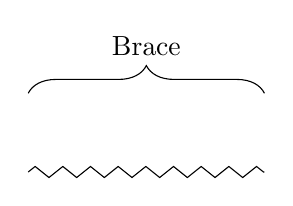
\begin{tikzpicture}
\draw[decorate, decoration={brace, amplitude=10pt}] (0,0) -- (3,0) node[midway, above=10pt] {Brace};
\draw[decorate, decoration={zigzag, amplitude=2pt}] (0,-1) -- (3,-1);
\end{tikzpicture}

\subsection{Shadows and Effects}
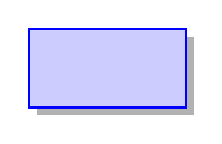
\begin{tikzpicture}
% Simulated drop shadow using a filled, slightly offset rectangle
\fill[black, opacity=0.3] (0.1,-0.1) rectangle (2.1,0.9);
\draw[fill=blue!20, draw=blue, thick] (0,0) rectangle (2,1);
\end{tikzpicture}

\section{Best Practices for TikZ}
\begin{itemize}
    \item Use relative coordinates when possible
    \item Define styles for consistent formatting
    \item Use meaningful node names
    \item Keep diagrams simple and clear
    \item Use appropriate line weights and colors
    \item Test diagrams at different scales
\end{itemize}

\section{Reference Examples from Dr. Trefor Bazett's Tutorial}
The following examples are directly from the tutorial video demonstrating key TikZ concepts as taught by Dr. Trefor Bazett. These examples showcase the fundamental patterns used throughout the tutorial.

\subsection{Example 1: Drawing and Styling a Circle}
This example demonstrates basic drawing commands and styling options. It shows how to:
\begin{itemize}
    \item Draw a horizontal line connecting two points
    \item Apply multiple styling options (dashed, color, thickness) to a circle
    \item Use square brackets to specify style parameters
\end{itemize}

\begin{center}
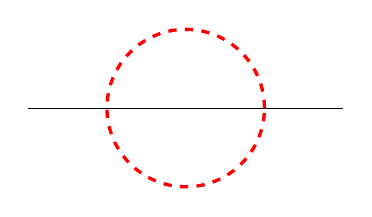
\begin{tikzpicture}
    % Draw a line from (0,0) to (4,0)
    \draw (0,0) -- (4,0);

    % Draw a dashed red circle with a center at (2,0) and a radius of 1cm
    \draw[dashed, red, very thick] (2,0) circle (1cm); 
\end{tikzpicture}
\end{center}

Key concepts: The \texttt{draw} command, coordinate specification, and style parameters in square brackets.

\subsection{Example 2: Defining and Using Custom Styles}
This example creates a reusable style called \texttt{sir} and uses it to draw diagram boxes with styled nodes. This demonstrates:
\begin{itemize}
    \item How to define custom styles in the tikzpicture options
    \item Using the positioning library with \texttt{below of}
    \item Connecting nodes by referencing their names and anchors
    \item Setting node distance for consistent spacing
\end{itemize}

\begin{center}
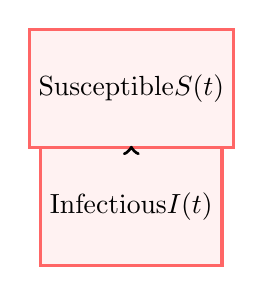
\begin{tikzpicture}[
    sir/.style={
        rectangle, 
        draw=red!60!white, 
        fill=red!5!white, 
        very thick, 
        minimum size=1.5cm
    },
    % Positioning library is required for 'below of'
    node distance=1.5cm 
]

    % Create the first node (Susceptible)
    \node[sir] (susceptible) {Susceptible \\ $S(t)$}; 

    % Create the second node (Infectious) positioned below the first
    \node[sir, below of=susceptible] (infectious) {Infectious \\ $I(t)$};

    % Draw a very thick arrow between the two nodes
    \draw[->, very thick] (susceptible.south) -- (infectious.north);

\end{tikzpicture}
\end{center}

Key concepts: Custom style definition, node naming, relative positioning with \texttt{below of}, and anchor-based connections (\texttt{.south}, \texttt{.north}).

\subsection{Example 3: Complex Diagram with Multiple Node Relationships}
This example extends the concepts to show a more complete diagram with multiple nodes and connection types:

\begin{center}
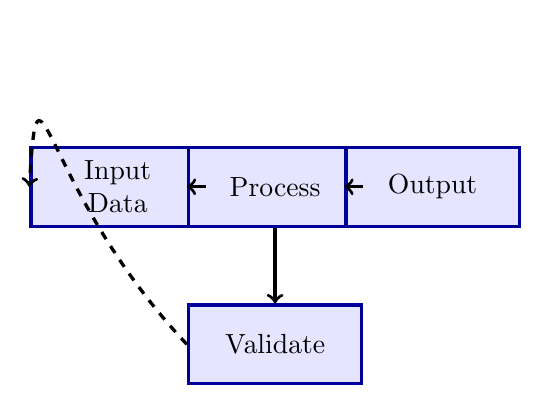
\begin{tikzpicture}[
    box/.style={
        rectangle, 
        draw=blue!60!black, 
        fill=blue!10, 
        very thick, 
        minimum width=2.2cm,
        minimum height=1cm,
        align=center
    },
    node distance=2cm
]
    % Define nodes
    \node[box] (input) {Input \\ Data};
    \node[box, right of=input] (process) {Process};
    \node[box, right of=process] (output) {Output};
    \node[box, below of=process] (validate) {Validate};
    
    % Straight arrows
    \draw[->, very thick] (input) -- (process);
    \draw[->, very thick] (process) -- (output);
    \draw[->, very thick] (process) -- (validate);
    
    % Curved arrow using Bézier control points
    \draw[->, very thick, dashed] (validate.west) 
        .. controls (-1,0) and (-1,2) .. 
        (input.west);
\end{tikzpicture}
\end{center}

This shows how to create feedback loops and complex flows using both straight and curved connections.

\end{document}
